\section{Uppdragsgivare och resurser}
I det här kapitlet går vi in djupare på
vilka uppdragsgivarna är, samt den prototyp vi har tagit del av. Kapitlet ska ge dig som läsare en bakgrund för att förstå rapporten bättre.  

\subsection{VNTRS}
VNTS är ett konsultbolag som har sin bas i Stockholm. VNTRS grundades av fyra managementkonsulter. Deras vision är att hjälpa entreprenörer samt stora företag med innovativa digitala produkter och tjänster. VNTRS har i nuläget, Maj 2018, 21 anställda i sitt bolag. De har junior samt seniora konsulter som har erfarenhet inom iOS-utveckling, Android-utveckling, Frontend-utveckling, Backend- och UX / UI-utveckling tillsammans med personer som arbetar med marknadsstrategi. De hjälper sina kunder att utveckla en del i eller en hel digitala produkt eller tjänst, beroende på behov och uppdrag. VNTRS har utvecklat digitala produkter så som Byt Grej, Zipo, SUNI och BakingHood\cite{VNTRSAB}och har arbetat med bolag som Office Depot, NRK och Husbanken. 

\subsection{Amazing Leaders}
I den här studien är vår uppdragsgivare Amazing Leaders, där deras jobb går ut på att möjliggöra framgångsrikt ledarskap med hjälp av individers emotionella talang. De jobbar med kunder som exempelvis Telia, SEB och Adidas där de arbetar tillsammans med kund för att engagera och få en ledareffektivitet. Termen EQ-smart är något de lyfter fram där de tillsammans med diverse program vill öka individers emotionella intelligens. Emotionell intelligens kan handla om ens förmåga att kunna känna igen och kontrollera känslor hos en själv och andra. Amazing Leaders EQ ramverk är baserat på psykologen Martyn Newmans definition och forskning om EQ. Detta ramverk skapade en röd tråd inom Amazing Leaders där de arbetar med att utveckla människors och verksamheters emotionella intelligens, för att nå hållbara resultat. 
\newline

De menar på att för att få ett högpresterande team och en ledareffektivitet behöver man jobba på EQ. De har tjänster som individuell coachning, teamutveckling, ledarskapsprogram, karriärcoachning för att nämna några. De åstadkommer att utbilda individer om EQ genom digiloga processer, där man har mänskliga möten med digitalt stöd. Genom att jobba med EQ har de kunnat jobba med den forskningen som fanns vilket har möjliggjort att mäta resultat kopplat till deras kunders KPI:er (Keep Performance Index). Idag har deras rapporter och resultat visat på att emotionellt starka människor är bättre ledare som i sin tur skapar effektivare och konkurrenskraftigare företag. {\cite{AmazingLeaders2017OmLeaders}}
\newline

\subsection{AL1 - prototypen}
Den prototyp som använts i denna studie har utformats av VNTRS. AL1 innehåller i sin helhet en video på en av Amazing Leaders' coacher, Ursula. Syftet med prototypen var att få en inblick i hur den framtida applikationen skulle komma att se ut. Prototypen börjar med att Ursula pratar informativt om värderingar. Sedan får användaren stegvis svara på olika frågor under videons gång. Användaren får svara på frågor genom att klicka i förvalda alternativ på en skala samt genom att själv få skriva i sina svar. I slutet visas en graf som ska representera dina värderingar baserat på vad du som användare har svarat.
\newline

\begin{figure} [H] 
  \centering
  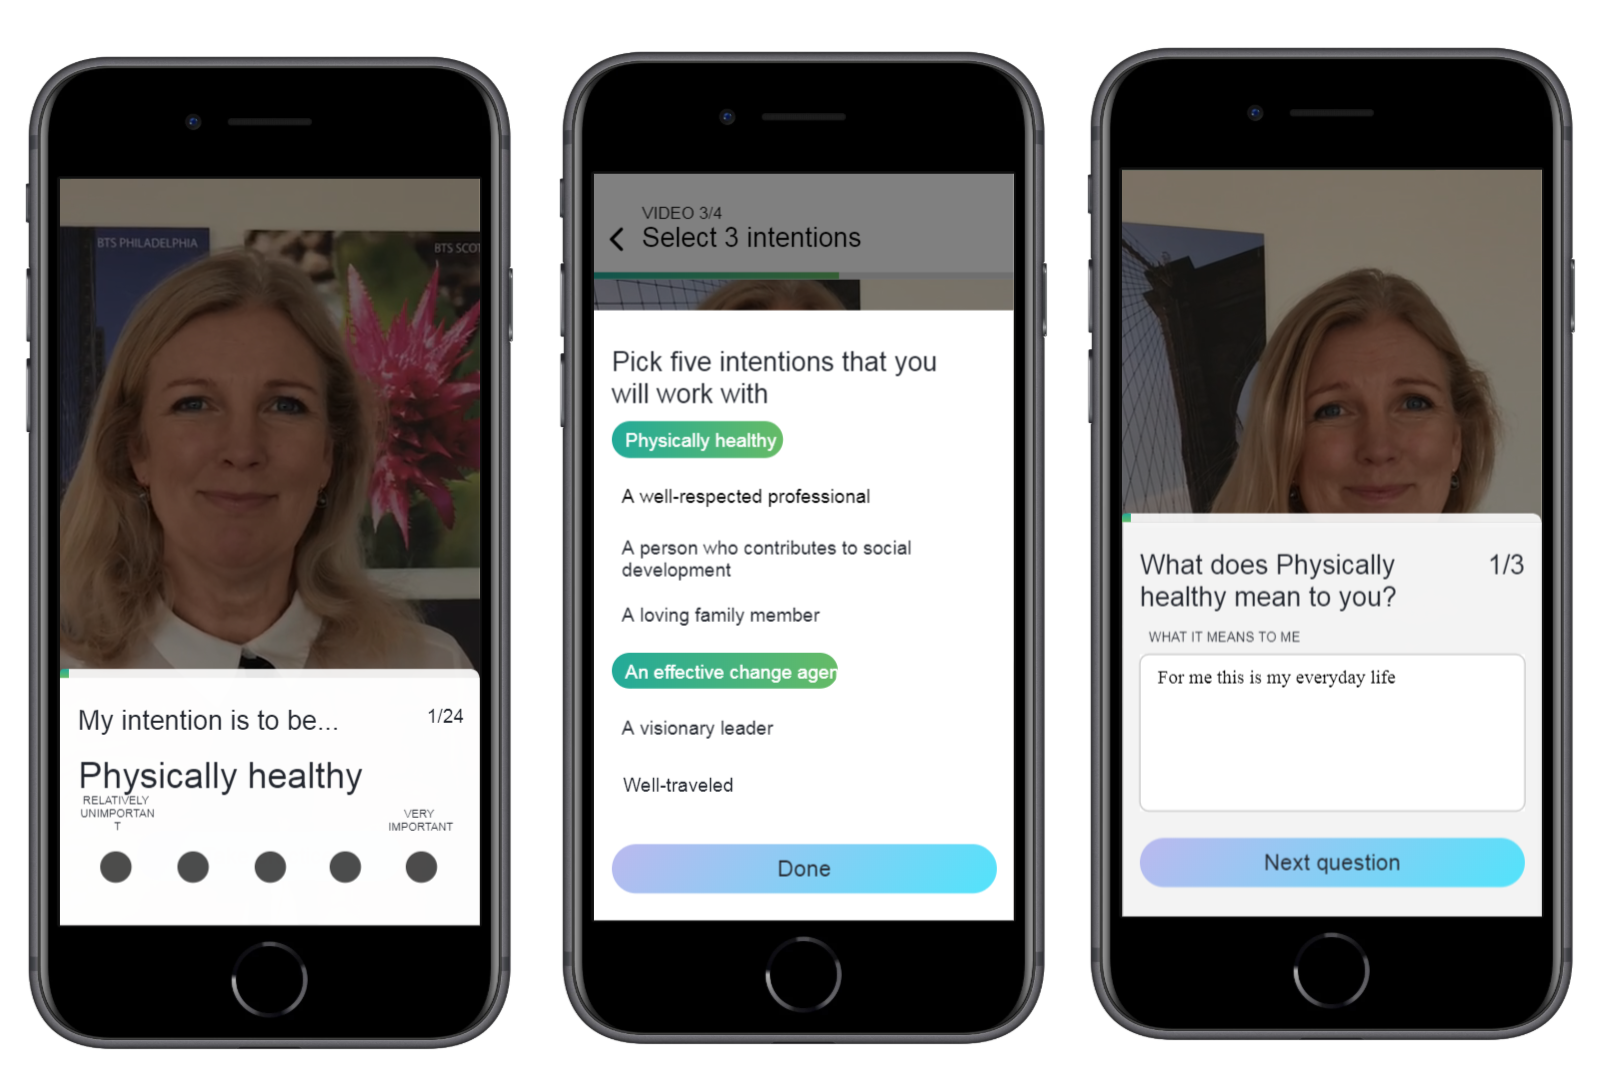
\includegraphics[scale=0.3]{AL1.png}
\centering
\captionsetup{justification=centering,margin=2cm}
\caption{Bild på AL1 som visar olika svarsalternativ}
\end{figure} 
Prototypen har som tydligt mål att användas i syfte av att testa användarupplevelsen, det vill säga den övergripande interaktionen som testperson har med prototypen. Besläktade testområden som användbarheten utesluts från prototypens ändamål. Eftersom att det fanns en risk att prototypen hade brister, utbildades testpersoner kort om distinktionerna mellan användbarhet och användarupplevelse. 
\newline

